\documentclass[a4paper]{scrartcl}
\usepackage{amssymb}
\usepackage{amsmath}
\usepackage{hyperref}
\usepackage{graphicx}
\usepackage{pgfgantt}

\begin{document}

\title{A Probabilistic Model for Software Defect Prediction}
\subtitle{Thesis Proposal}
\author{James Tunnell}
\maketitle

\section{Introduction}
Search-Based Software Engineering (SBSE) is an emerging area of research, where search-based optimization techniques are applied to the Software Engineering problem domain. SBSE problems include The Next Release Problem, Structural Test Data Generation, and Software Cost Estimation\cite{2012_harman_search}.

To make SBSE of practical use on a software project, a method is needed to model the practical details of a project in an abstract way so that is amenable to search-based optimization. In this paper, such a model is developed toward making use of algorithms developed for the Next Release Problem (NRP).

In the NRP, proposed features have an associated cost, so that an optimal feature subset can be selected. Now it might be suggested that the estimated cost of a proposed feature can be used directly in a NRP algorithm. But, there is a practical detail that prevents this: the total cost of a feature includes both the cost of implementation \emph{and} the cost of fixing associated defects.

Of course, defects that will be associated with a feature are not known in advance, so determining their exact cost would be impossible. But if associated defects can be predicted, then the cost of such defects can be estimated.

To this end, a model is proposed for predicting the defects associated with some proposed feature, with some level of confidence. The model will be probabilistic, and will be built using a software project's historical data, available from an issue tracking database.

Exploratory data analysis was conducted on a software project, \href{https://www.mongodb.org}{MongoDB}, in order to asses the feasibility of such a predictive model.

The remainder of this document is organized as follows. First, the \nameref{sec:background} section provides details on the Next Release Problem and the methods used software project data collection. Next, the \nameref{sec:related_work} section describes other approaches used in defect prediction, which mainly center around static code analysis. Then, the \nameref{sec:exploratory} section presents the  methods used, and results obtained for exploratory data analysis. Finally, the \nameref{sec:proposed_work} section lays out the specific tasks that are proposed in order to design an effective predictive model, in the context of the results obtained from exploratory data analysis.

\section{Background}
\label{sec:background}
In this section, first the Next Release Problem will be introduced and described more formally. Then, the methods used for collecting historical data from software projects will be discussed.

\subsection{The Next Release Problem (NRP)}
The Next Release Problem (NRP) was defined by Bagnall et al\cite{2001_bagnall_nrp}, and was shown to be NP-Hard. Being abstract in its treatment of feature cost, a broad range of optimization techniques can be applied to the NRP, such as integer programming, hill climbing, simulated annealing, genetic algorithms, etc. The NRP is the subject of academic research in the area of Search-Based Software Engineering\cite{2010_jiang_hybrid,2012_xuan_solving,2007_zhang_multi_obj_nrp}.

The NRP is designed to aid software project planners, who have multiple customers to satisfy. The project planner would like to maximize the revenue produced from completing the project. This is all described mathematically as follows.

A software project has a set $R$ of all possible requirements (new features and enhancements) that might be included in the next software release. A customer $i$ is satisfied by completing a subset $R_i \subseteq R$. The importance of a customer $i$ is given by the weight, $w_i \in \mathbb{Z}^+$.

Requirements may have acyclic dependencies, or prerequisites, that must be completed first. A subset that includes all prerequisite requirements, recursively, is indicated by $\hat{R}_i$, and should be taken to mean
\begin{equation}
\hat{R}_i = R_i \cup ancestors(R_i)
\end{equation}

For example, if $R_1 = \{r_2\}$, and $r_1$ is a prerequisite for $r_2$, then $\hat{R}_1 = \{r_1,r_2\}$.

A requirement $r \in R$ has a cost $cost(r) \in \mathbb{Z}^+$, associated with its implementation, not considering the cost of any prerequisite requirements. Then, the cost for some subset $R' \subseteq R$ will be
\begin{equation}
cost(R') = \sum \{cost(r) | r \in \hat{R}_i \}
\end{equation}

Once customer $i$ is satisfied, their weight $w_i$ contributes to the total revenue from the project, as in
\begin{equation}
\sum_{i \in S} w_i
\end{equation}

So, the NRP is posed as follows: for a group of $n$ customers, select the subset $S \subseteq \{ 1,2,...,n \}$ that maximizes total revenue, while keeping the total cost within some budget constraint $B$. This is given by 
\begin{equation}
\begin{split}
maximize~~& \sum_{i \in S} w_i \\
subject~to~~~& cost(\bigcup_{i \in S} \hat{R}_i) \le B
\end{split}
\end{equation}

\subsection{Issue Tracking Systems}
The empirical data used to establish a predictive model will be taken from software project historical data, found in an Issue Tracking System (ITS). In addition to tracking bugs, past and present, an ITS can be used to track features, enhancements, or any other type of software process issue. 

\subsubsection{JIRA}
\href{https://www.atlassian.com/software/jira}{JIRA} is product by \href{https://www.atlassian.com/}{Atlassian} that provides issue/bug tracking and project management features. For qualified open source projects, Atlassian will provide a JIRA subscription for free.

\section{Related Work}
\label{sec:related_work}

Software defect (bug) prediction typically involves a detailed analysis of code or proposed design changes. Akiyama \cite{1971_akiyama} predicted defect counts based on lines of code (LOC), number of decisions, and the number of subroutine calls. Gafney \cite{1984_gaffney_estimating} likewise predicted defect count based on LOC. Rather than code itself, Henry and Kafura \cite{1984_henry_evaluation} define metrics that are based on information taken from design documents, to be used in defect prediction.

TODO: discuss more about the above methods

\subsection{Other Approaches to Defect Projection}
Rather than requiring a detailed code analysis to predict defects, the approach proposed in this paper is to develop a mathematical model based on historical data on defect occurrences. Specifically, the proposed approach is to develop a prediction model using software features as inputs and defects as outputs.

A related approach, used by Li et al.\cite{2004_li_emperical_eval}, is to study only the defect occurrences themselves, and attempt to develop a mathematical model for defect projection. In their work, functions were fitted to a time series of defect occurrences, then the function parameters themselves were extrapolated for each new release. They found that the Weibull model fit best in 73\% of the tested software releases. They attempted to extrapolate model parameters using naïve methods, moving averages, and exponential smoothing, but found these techniques to be "...inadequate in extrapolating model parameters of the Weibull model for defect-occurrence projection". The reason given for this ineffectiveness is the changing nature of the software development system For example, development practices, staffing levels, and usage patterns may all change between releases.

In another related approach, Graves et al.\cite{2000_graves_predicting} develop several models that predict the future distribution of software faults in a given code module. The basis of their predictive models is a statistical analysis of change management data, which describes only the changes made to code files. The best model they found, was a weighted time damp model, where every change in the module files contributed to fault prediction, with time-damping to account for age of changes. They achieved "slightly less successful performance" by basing a generalized linear model on just the modules age and the number of past changes. They also found factors that did not improve model performance: module length, number of developers making changes in the module, and how often a module is changed simultaneously with another module.

\section{Exploratory Data Analysis}
\label{sec:exploratory}
This section covers the exploratory data analysis which was performed to asses the feasibility of developing a predictive model for software defects. In this section, first the methods used to collect and analyze the data are presented. Then the analysis results are presented and interpreted.

\subsection{Data Collection}
The MongoDB project was selected for exploratory data analysis. The criteria for project selection, and also the methods used, are explained in the following subsections.

\subsubsection{Project Select Criteria}
To facilitate data collection, only projects that have a freely accessible Issue Tracking System (ITS) were considered. Included in this category are open-source software projects. Also, only projects with a consistent and transparent release policy were considered. Last, a long history of project data was an important consideration. MongoDB met all these considerations.

\subsubsection{Data Collection Methods}
Data collection is semi-automatic. First, there is a manual step is to export data from JIRA as XML. This was performed by using the \href{https://jira.mongodb.org}{Web interface for the MongoDB JIRA server}. Then, pertinent data is automatically extracted using a Python script. 

\subsubsection{Data Transformation}
Once extracted, data undergoes some transformation before analysis. First, because \textit{Sub-task} issues are related to their parent issue, each subtask is converted to an issue with the same type as its parent. Next, in order to compare issues that have the same type and priority, an additional \textit{time-to-resolve} field is derived. This  is done simply by calculating the difference (in days) between \textit{date-created} and \textit{date-resolved}.

\subsubsection{Data Format}
Once the data is collected, extracted, and transformed, it is finally saved in a text file as a table for later analysis in R. The columns in this table are: type, priority, and time-to-resolve (in days).

\subsection{Data Analysis}
Historical data from each software project was analyzed over both the long term (all releases) and short term (each significant\footnote{For the MongoDB project, a significant release period is comprised of an odd/even-versioned release pair (e.g. 2.1 and 2.2). The odd-versioned release is unstable, for development work, and the even-versioned release is for bug-fixing only.} release period). The long-term analysis will provide an overview of each project, and possibly reveal some consistent patterns between projects. The short-term analysis will serve to isolate each significant release period as a cause-and-effect period (changes being the causes, and bugs being the effects).

Before presenting the results of data analysis, next the data analysis methods are discussed.

\subsubsection{Data Analysis Methods}
Project historical data was analyzed as follows. First, for each period of analysis, data was be separated by category: first, by issue type, and then by priority. The remaining data attribute was the time to resolve (in days). Once separated, each data group was summarized using frequency count and descriptive statistics, represented visually and numerically. Last, a good-fitting probability distribution was found for each data group, and shown set against a histogram of the data.

\subsection{Results}
The analysis results presented are broken up into subsections for long-term and short-term analysis. Following each will be interpretation of the results.

\subsubsection{Long-term Analysis Results}
In this long-term analysis, data from all releases are put together for analysis. This set of data is then broken down into subgroups by type and priority.

First, descriptive statistics are presented, which include frequency count, and the following summary statistics: minimum, 1st quartile, median (2nd quartile), 3rd quartile, mean, and maximum.

\begin{table}[h!]
\caption{Frequency of issues, by type and by priority}
\centering
\begin{tabular}{ r | c | c | c | c |  c | }
\hline
~ & \multicolumn{5}{|c|}{Priority} \\
Type & 1 & 2 & 3 & 4 & 5 \\
\hline\hline
Bugs & 62 & 239 & 2759 & 484 & 87 \\
Improvements & 1 & 28 & 1026 & 300 & 71 \\
New Features & 1 & 3 & 229 & 46 & 7 \\
Questions & 0 & 0 & 25 & 9 & 0 \\
Tasks & 1 & 7 & 192 & 28 & 8 \\
\hline
\end{tabular}
\label{tab:all_freqcount}
\end{table}


\begin{figure}
\begin{center}
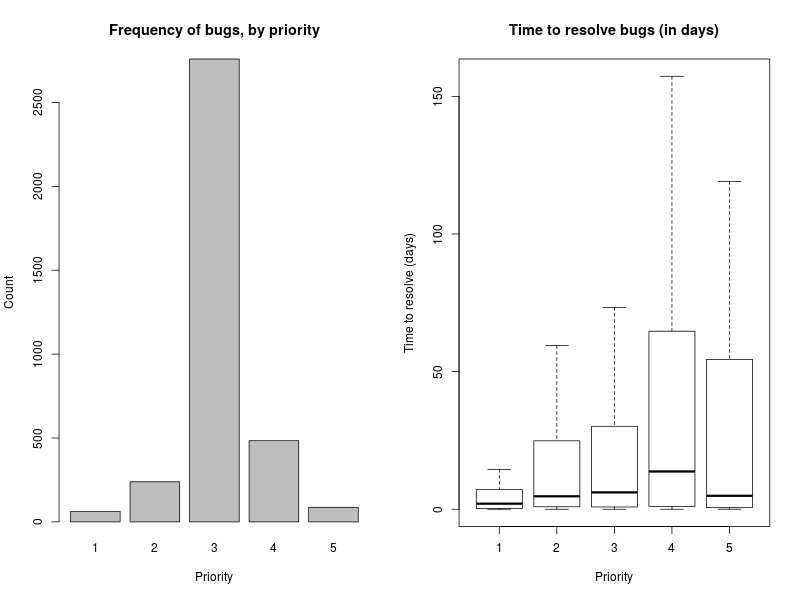
\includegraphics[width=6in]{exploratory_results/mongodb_allreleases/bugs}
\caption{Descriptive statistics of bugs from all releases, by priority}
\label{fig:all_bugs}
\end{center}
\end{figure}

\begin{table}[h!]
\caption{Summary statistics of bugs, by priority}
\centering
\begin{tabular}{ r | l | l | l | l |  l | l }
\hline
Priority & Min. & 1st Qu. & Median & Mean & 3rd Qu. & Max. \\
\hline\hline
1 & 0.00046 & 0.36710 & 2.01700 & 11.42000 & 7.10000 & 118.60000 \\
2 & 0.0001 & 0.8911 & 4.6930 & 44.9600 & 24.8400 & 902.1000 \\
3 & 0.0000 & 0.8247 & 6.1120 & 43.3000 & 30.1200 & 1365.0000 \\
4 & 0.000 & 1.034 & 13.710 & 73.640 & 64.390 & 1300.000 \\
5 & 0.0017 & 0.6199 & 4.8780 & 63.7800 & 54.4400 & 560.0000 \\
\hline
\end{tabular}
\label{tab:all_bugs_summary}
\end{table}

\begin{figure}
\begin{center}
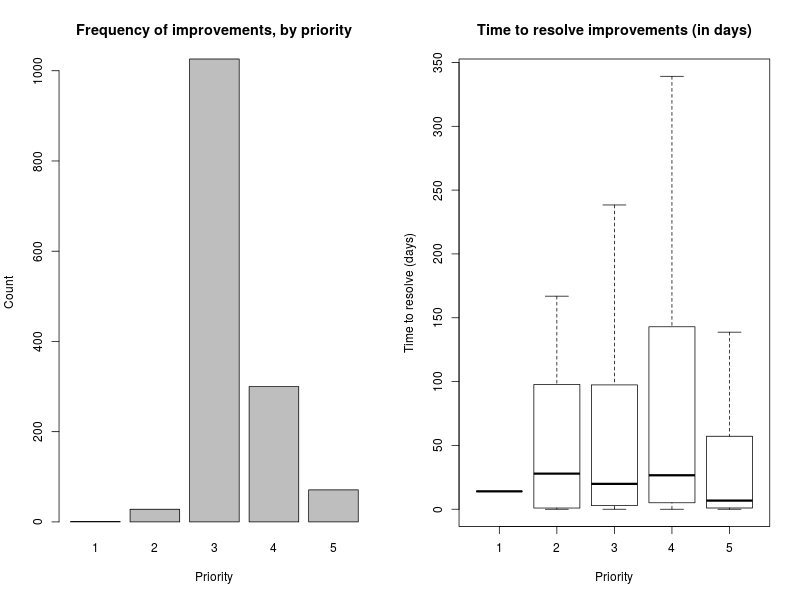
\includegraphics[width=6in]{exploratory_results/mongodb_allreleases/improvements}
\caption{Descriptive statistics of improvements from all releases, by priority}
\label{fig:all_improvements}
\end{center}
\end{figure}

\begin{table}[h!]
\caption{Summary statistics of improvements, by priority}
\centering
\begin{tabular}{ r | l | l | l | l |  l | l }
\hline
Priority & Min. & 1st Qu. & Median & Mean & 3rd Qu. & Max. \\
\hline\hline
1 & 14 & 14 & 14 & 14 & 14 & 14 \\
2 & 0.0025 & 0.9847 & 27.8800 & 85.8900 & 92.8100 & 621.2000 \\
3 & 0.000 & 2.869 & 19.840 & 101.700 & 97.250 & 1429.000 \\
4 & 0.000 & 5.053 & 26.590 & 114.600 & 142.600 & 1380.000 \\
5 & 0.0014 & 0.9455 & 6.7270 & 63.3000 & 57.1500 & 786.1000 \\
\hline
\end{tabular}
\label{tab:all_improvements_summary}
\end{table}

\begin{figure}
\begin{center}
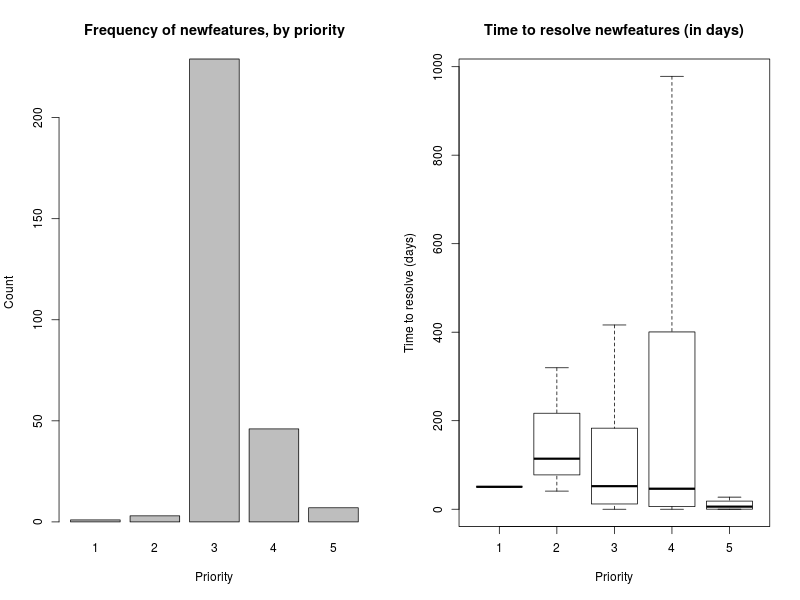
\includegraphics[width=6in]{exploratory_results/mongodb_allreleases/newfeatures}
\caption{Descriptive statistics of new features from all releases, by priority}
\label{fig:all_newfeatures}
\end{center}
\end{figure}

\begin{table}[h!]
\caption{Summary statistics of new features, by priority}
\centering
\begin{tabular}{ r | l | l | l | l |  l | l }
\hline
Priority & Min. & 1st Qu. & Median & Mean & 3rd Qu. & Max. \\
\hline\hline
1 & 50.65 & 50.65 & 50.65 & 50.65 & 50.65 & 50.65 \\
2 & 40.95 & 77.54 & 114.10 & 158.20 & 216.90 & 319.60 \\
3 & 0.0001 & 11.8200 & 52.0700 & 157.1000 & 183.2000 & 1287.0000 \\
4 & 0.0001 & 6.0340 & 46.3200 & 260.1000 & 384.6000 & 1416.0000 \\
5 & 0.01487 & 0.14220 & 5.81200 & 23.23000 & 18.37000 & 119.80000 \\
\hline
\end{tabular}
\label{tab:all_newfeatures_summary}
\end{table}

\begin{figure}
\begin{center}
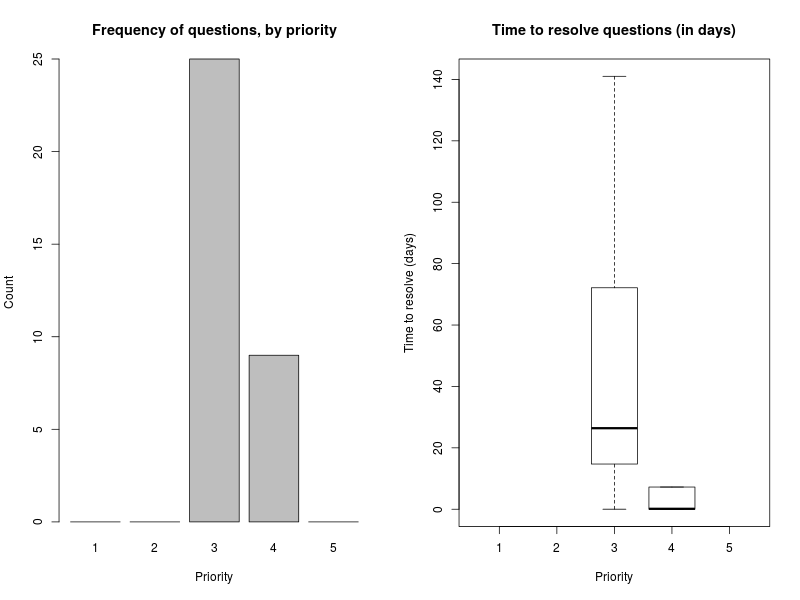
\includegraphics[width=6in]{exploratory_results/mongodb_allreleases/questions}
\caption{Descriptive statistics of questions from all releases, by priority}
\label{fig:all_questions}
\end{center}
\end{figure}

\begin{table}[h!]
\caption{Summary statistics of questions, by priority}
\centering
\begin{tabular}{ r | l | l | l | l |  l | l }
\hline
Priority & Min. & 1st Qu. & Median & Mean & 3rd Qu. & Max. \\
\hline\hline
3 & 0.0017 & 14.7200 & 26.3800 & 152.5000 & 72.1300 & 1106.0000 \\
4 & 0.00009 & 0.01155 & 0.13950 & 54.83000 & 7.23100 & 271.80000 \\
\hline
\end{tabular}
\label{tab:all_questions_summary}
\end{table}

\begin{figure}
\begin{center}
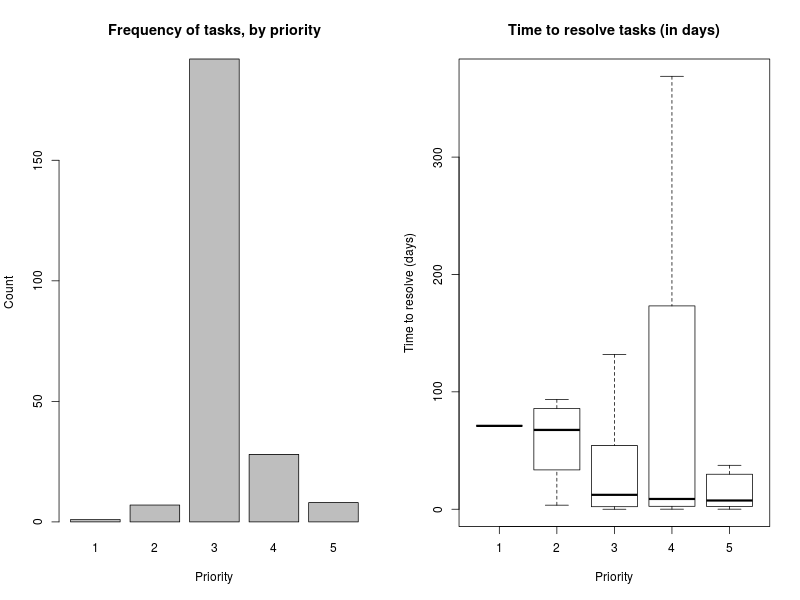
\includegraphics[width=6in]{exploratory_results/mongodb_allreleases/tasks}
\caption{Descriptive statistics of tasks from all releases, by priority}
\label{fig:all_tasks}
\end{center}
\end{figure}

\begin{table}[h!]
\caption{Summary statistics of tasks, by priority}
\centering
\begin{tabular}{ r | l | l | l | l |  l | l }
\hline
Priority & Min. & 1st Qu. & Median & Mean & 3rd Qu. & Max. \\
\hline\hline
1 & 71.02 & 71.02 & 71.02 & 71.02 & 71.02 & 71.02 \\
2 & 3.453 & 33.510 & 67.560 & 121.100 & 85.820 & 537.800 \\
3 & 0.0013 & 2.1460 & 12.2600 & 60.4400 & 53.6000 & 1436.0000 \\
4 & 0.0315 & 2.6080 & 8.7250 & 84.0500 & 169.5000 & 368.8000 \\
5 & 0.05017 & 3.11400 & 7.41800 & 23.31000 & 26.03000 & 107.10000 \\
\hline
\end{tabular}
\label{tab:all_tasks_summary}
\end{table}

\subsubsection{Short-term Analysis Results}
TODO

\section{Proposed Work}
\label{sec:proposed_work}

The Next Release Problem (NRP) is not readily applicable to the release planning process in a software project. This is due to the abstract nature of the NRP. But by modelling the practical details of release planning, the way could be paved for making use of optimization techniques already developed for the NRP.

Feature cost is a critical part of the NRP. An inaccurate cost estimate might mislead a project planner into believing that a feature subset can be implemented inside the budgeted constraint when that may not be the case. And because the cost of fixing defects contributes to the total cost of a feature, the cost of fixing defects should be accounted for.

To this end, the work proposed here is to develop a model for predicting the defects associated with some proposed feature, with some level of confidence. The model will be probabilistic, and will be built using the same data collected for \nameref{sec:exploratory}.

The breakdown of this work, and the timeline for completing it are discussed next.

\subsection{Modelling Work}
The modelling work itself can broken up as follows:
\begin{enumerate}
\item
\textbf{Select candidate model structures}. There are potentially many different model structures that can be used. Several structures will be put forth as likely candidates for a model.
\item
\textbf{Optimize model parameters}. For each candidate model structure, parameters will be chosen using Maximum Likelihood Estimation (MLE).
\item
\textbf{Validate model}. Models will be validated by: TODO 
\end{enumerate}

\subsection{Timeline}
The proposed modelling work is to be completed over the winter quarter in 2015. A timeline of this work, along with the up-front work of forming a committee and presenting this proposal, is listed in Table \ref{tab:timeline} below.

\begin{table}[h]
\caption{Timeline for proposed work}
\centering
\begin{tabular}{ p{2.5in} l l}
\hline\hline
Task & Start Date & End Date \\
\hline
Form committee & Nov 10 & Dec 5 \\
Present proposal & Jan 6 & Jan 16 \\
Respond to committee feedback & Jan 19 & Jan 23 \\
Select candidate model structures & Jan 26 & Feb 13 \\
Optimize parameters and validate models & Feb 9 & Feb 27 \\
Repeat procedures for two more SW projects & Mar 2 & Mar 20 \\
\hline
\end{tabular}
\label{tab:timeline}
\end{table}

\appendix
\section{Software Requirements}
\label{sw_reqs}
The software developed so far has been used for data collection and analysis. The scripts used can be run on any platform that supports Python and R. Besides this basic requirement, here are the other dependencies:
\paragraph{Python dependencies:}
\begin{itemize}
\item
docopt: for defining command-line interfaces and parsers. See the \href{https://github.com/docopt/docopt}{GitHub page} for installation instructions.
\item
BeatifulSoup: for processing XML files. See the \href{http://www.crummy.com/software/BeautifulSoup}{support page} for installation instructions.
\end{itemize}

\paragraph{R dependencies:}
\begin{itemize}
\item
devtools: adds github\_install function. Install by running ``\verb|install.packages("devtools")|" on the R command line.
\item{docopt: for defining command-line interfaces and parsers. See the \href{https://github.com/edwindj/docopt.R}{GitHub page} for installation instructions.}
\end{itemize}


\bibliography{references}
\bibliographystyle{abbrv}

\end{document}